\chapter{Giới thiệu}
Mạng nơ ron sâu (DNNs) đã đạt hiệu quả rất tốt với các bài toán trong học máy
và trí tuệ nhân tạo như phân loại ảnh, nhận diện giọng nói, dịch máy và trò chơi.
Mặc dù DNNs rất hiệu quả nhưng một số nghiên cứu gần đây đã chứng minh DNNs rất 
dễ  "tổn thương" với các mẫu đối nghịch (Szegedy et al. 2013; Goodfellow, Shlens, 
and Szegedy 2015). Ví dụ, ảnh được gây nhiễu khéo có thể
làm cho một DNN đã được huấn luyện phân loại sai. Hơn nữa, các mẫu đối nghịch
được tạo ra hầu như không thể phân biệt được bằng mắt người. 
\begin{figure}[H] % places figure environment here   
    \centering % Centers Graphic
    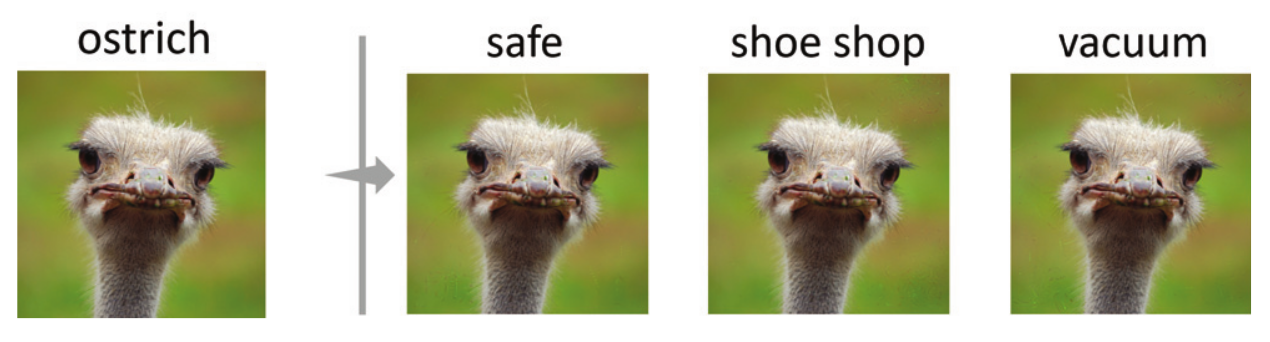
\includegraphics[width=0.8\textwidth]{assets/fig_01.png} 
    \caption{Minh họa trực quan về mẫu đối nghịch được sinh bởi EAD. 
    Hình gốc (đà điểu) được lấy từ tập ImageNet. Các mẫu đối nghịch bị 
    phân loại sai với mô hình Inception-v3.} % Creates caption underneath graph
    \label{fig:fg_01}
\end{figure}
Ví dụ trực quan trên thể hiện 3 mẫu đối nghịch của một hình con đà điểu ("ostrich") 
được sinh ra bằng thuật toán nhóm tác giả đề xuất. Các mẫu này được mô hình Inception-v3 
(Szegedy et al. 2016) phân loại thành "safe", "shoe shop" và "vacuum". 

Sự thiếu mạnh mẽ của DNN trước các mẫu đối nghịch đã làm dấy lên những lo ngại 
về vấn đề bảo mật các ứng dụng, bao gồm nhận dạng tín hiệu giao thông 
và phát hiện phần mềm độc hại. Hơn nữa, vượt ra ngoài không gian số, 
các nhà nghiên cứu đã chỉ ra rằng những mẫu đối nghịch ảnh hưởng cả tới thế giới thực trong việc đánh lừa DNNs (Kurakin, Goodfellow, and Bengio 2016a; Evtimov et al. 2017).
Do tính mạnh mẽ và ý nghĩa bảo mật, việc tạo ra các mẫu đối nghịch được gọi là 
tấn công (\textit{attacks}) vào DNNs. Cụ thể, tấn công nhắm đích 
(\textit{targeted attacks}) để tạo ra các mẫu đối nghịch được phân loại nhầm vào các lớp mục tiêu 
định sẵn; tấn công không nhắm đích (\textit{untargeted attacks}) để tạo ra các mẫu đối nghịch không được phân loại vào lớp ban đầu. Chuyển giao tấn công (\textit{transfer attacks}) nhằm mục đích tạo ra các mẫu đối nghịch có thể chuyển 
từ mô hình DNN này sang mô hình DNN khác. Ngoài việc đánh giá mức độ mạnh mẽ của DNNs,
các mẫu đối nghịch còn có thể được sử dụng để huấn luyện mô hình sao cho nó có khả năng chống chịu 
với những xáo trộn của đối nghịch, gọi là huấn luyện đối nghịch (\textit{adverarial training}) 
(Madry et al. 2017). Chúng cũng có thể được sử dụng để cải tiến DNNs (Koh và Liang 2017;
Dong et al. 2017). 

Trong bài báo này, tác giả sử dụng các mẫu đối nghịch để tấn công phân loại ảnh dựa trên 
mạng neuron tích chập. Mẫu đối nghịch được tạo ra để làm sai lệch kết quả dự đoán và phải đảm bảo
hình mới tạo ra (gần) giống với hình gốc. Trong trường hợp này, sự giống nhau giữa mẫu đối nghịch và hình gốc được đo bằng các độ đo nhiễu (\textit{distortion metrics}) khác nhau.
Độ đo thường được sử dụng là chuẩn $L_q$ 
với $\lVert x \rVert_q = \left( \sum_{i=1}^p |x_i|^q \right)^{\frac{1}{q}}$ kí hiệu chuẩn $L_q$
của vector $p$ chiều $x = [x_1, ..., x_p]$ với $q \geq 1$. Cụ thể, khi tạo ra các mẫu đối nghịch
, chuẩn $L_{\infty}$ được sử dụng để đánh giá sự thay đổi tối đa giá trị điểm ảnh (Goodfellow, 
Shlens, and Szegedy 2015), chuẩn $L_2$ được sử dụng để cải thiện chất lượng thị giác của 
ảnh (Carlini and Wagner 2017b). Mặc dù, chuẩn $L_1$ thực tế được sử dụng rộng rãi 
trong các bài toán chống nhiễu, khôi phục ảnh (Fu et al. 2006) cũng như phục hồi thưa (Candès and Wakin 2008), các mẫu đối nghịch dựa trên $L_1$ chưa được nghiên cứu nhiều. Trong bài toán mẫu đối nghịch,
độ biến dạng $L_1$ đánh giá tổng các thay đổi trong nhiễu và đóng vai trò là một thành phần
(hàm) lồi thay thế độ đo $L_0$, đo lường số lượng điểm ảnh bị nhiễu làm thay đổi (độ thưa). Để lấp đầy khoảng trống về mẫu đối nghịch $L_1$, nhóm tác giả đề xuất một thuật toán tấn công dựa trên hiệu chỉnh \textit{elastic-net}, được 
gọi là tấn công elastic-net vào DNNs (elastic-net attacks to DNNs - EAD). Hiệu chỉnh 
elastic-net là tổ hợp tuyến tính của các hàm phạt $L_1$ và $L_2$ và nó cũng là công cụ 
chuẩn cho bài toán lựa chọn thuộc tính đặc trưng cho dữ liệu nhiều chiều (Zou and Hastie 2005). 
Trong bài toán tấn công DNNs, EAD mở ra hướng nghiên cứu mới từ cách tấn công hiện đại dựa trên 
$L_2$ (Carlini and Wagner 2017b), nó tạo ra các mẫu đối nghịch dựa trên $L_1$ vừa hiệu quả hơn vừa khác biệt cơ bản với các phương pháp tấn công hiện có. 

Để khám phá hiệu quả của tấn công dựa trên $L_1$, nhóm tác giả tiến hành các thử nghiệm trên tập 
dữ liệu MNIST, CIFAR10, và ImageNet trong các tình huống tấn công khác nhau. So với các 
phương pháp tấn công hiện có dựa trên $L_2$ và $L_{\infty}$ (Kurakin, Goodfellow, and 
Bengio 2016b; Carlini and Wagner 2017b), EAD có thể đạt được tỉ lệ tấn công thành công tương 
tự khi phá vỡ DNNs được phòng thủ hoặc không phòng thủ (Papernot et al. 2016b). Quan trọng 
hơn, tác giả chỉ ra rằng, tấn công $L_1$ đạt được hiệu suất vượt trội so với các tấn
công $L_2$ và $L_{\infty}$ trong chuyển giao tấn công và huấn luyện đối nghịch bổ sung. Với tập dữ liệu khó nhất (MNIST), EAD cải thiện khả năng chuyển 
giao tấn công từ DNN không phòng thủ vào DNN được phòng thủ chắt lọc (defensively distilled DNN) đạt tỉ lệ thành công gần $99\%$. Thêm vào 
đó việc huấn luyện kèm theo với mẫu đối nghịch dựa trên $L_1$ và $L_2$ có thể tăng cường khả 
năng chống chịu của DNNs đối với các nhiễu loạn. Những kết quả này cho thấy EAD mang lại tập 
mẫu đối nghịch khác biệt nhưng hiệu quả hơn. Ngoài ra, đánh giá các tấn công dựa trên 
độ nhiễu $L_1$ cung cấp thêm hiểu biết mới về học máy đối kháng và sự bảo mật của DNNs, gợi 
ý rằng $L_1$ có thể bổ sung cho $L_2$ và $L_{\infty}$ thúc đẩy các framework về học máy đối 
kháng hoàn thiện hơn.
